
% ===========================================================================
% Title:
% ---------------------------------------------------------------------------
% to create Type I fonts type "dvips -P cmz -t letter <filename>"
% ===========================================================================
\documentclass[11pt]{article}       %--- LATEX 2e base
\usepackage{latexsym}               %--- LATEX 2e base
%---------------- Wide format -----------------------------------------------
\textwidth=6in \textheight=9in \oddsidemargin=0.25in
\evensidemargin=0.25in \topmargin=-0.5in
%--------------- Def., Theorem, Proof, etc. ---------------------------------
\newtheorem{definition}{Definition}
\newtheorem{theorem}{Theorem}
\newtheorem{lemma}{Lemma}
\newtheorem{corollary}{Corollary}
\newtheorem{property}{Property}
\newtheorem{observation}{Observation}
\newtheorem{fact}{Fact}
\newenvironment{proof}           {\noindent{\bf Proof.} }%
                                 {\null\hfill$\Box$\par\medskip}
%--------------- Algorithm --------------------------------------------------
\newtheorem{algX}{Algorithm}
\newenvironment{algorithm}       {\begin{algX}\begin{em}}%
                                 {\par\noindent --- End of Algorithm ---
                                 \end{em}\end{algX}}
\newcommand{\step}[2]            {\begin{list}{}
                                  {  \setlength{\topsep}{0cm}
                                     \setlength{\partopsep}{0cm}
                                     \setlength{\leftmargin}{0.8cm}
                                     \setlength{\labelwidth}{0.7cm}
                                     \setlength{\labelsep}{0.1cm}    }
                                  \item[#1]#2    \end{list}}
                                 % usage: \begin{algorithm} \label{xyz}
                                 %        ... \step{(1)}{...} ...
                                 %        \end{algorithm}
%--------------- Figures ----------------------------------------------------
\usepackage{graphicx}

\newcommand{\includeFig}[3]      {\begin{figure}[htb] \begin{center}
                                 \includegraphics
                                 [width=4in,keepaspectratio] %comment this line to disable scaling
                                 {#2}\caption{\label{#1}#3} \end{center} \end{figure}}
                                 % usage: \includeFig{label}{file}{caption}
%---------------Math--------------------------------------------------------
\usepackage{mathtools}
\DeclarePairedDelimiter{\ceil}{\lceil}{\rceil}
\DeclarePairedDelimiter{\floor}{\lfloor}{\rfloor}

%--------------Images------------------------------------------------------
\usepackage{graphicx}
\graphicspath{ {Figures/} }



% ===========================================================================
\begin{document}
% ===========================================================================

% ############################################################################
% Title
% ############################################################################

\title{Accurately computing large floating-point numbers using parallel computing}


% ############################################################################
% Author(s) (no blank lines !)
\author{
% ############################################################################
Tanvir Kaykobad\\
School of Computer Science\\
Carleton University\\
Ottawa, Canada K1S 5B6\\
{\em TanvirKaykobad@cmail.carleton.ca}
% ############################################################################
} % end-authors
% ############################################################################

\maketitle

% ############################################################################
% Abstract
% ############################################################################
\begin{abstract}
Parallel algorithms for accurately summing floating-point numbers are investigated and one is implemented. Primarily Goodrich et al.'s superaccumulator mapreduce algorithm is analyzed and the performance of the algorithm is compared.
\end{abstract}


% ############################################################################
\section{Introduction} \label{intro}
% ############################################################################

Addition of floating point numbers is nonassociative. The problem of addition of large number of floating point numbers arises when, for example, we need to find dot product of vectors having large number of coordinates. largehere are SIMD algorithms for accurately summing up very large number of small and large floating point numbers in parallel. It is known that for accurately summing up such a set of numbers one has to use snowball effect to obtain larger numbers from smaller ones. This idea is explored to see if it can be extended in parallel computing by introducing a huffman-tree like structure to pair floating point numbers of similar magnitude so that they can be summed up more accurately, ensuring minimum rounding error in the worst case while compromising as little as possible in non-parallel computation time. However, no non-heuristic algorithm currently exists for parallelizing Huffman-tree computation. Thus I have opted for implementing and testing the existing state of the art algorithm provided by Goodrich and Eldawy \cite{PASFPN} My implementation has been similar to that of Goodrich's, however I have summed the carry bit afterwards which requires an iteration of all the digits in the resulting number that Goodrich avoided.


% ############################################################################
\section{Literature Review} \label{litrev}
% ############################################################################

Demmel and Nguyen \cite{PRS} used Rump’s algorithm for floating point summation that is reproducible independent of the order of summation that may be different with the dynamic scheduling of parallel computing resources and floating point non-associativity. Their absolute error bound is $2^{-28}$ times macheps, and requires constant amount of extra memory usage. Demmel and Hida \cite{AEFPS} analysed several algorithms and showed that if a wider accumulator of F bits is used to sum n floating point numbers each of at most f bits, and if sum is carried out in descending order of exponents then an error of at most 1.5 times the least significant bit can occur provided that number of summands does not exceed $2^{(F-f)}$.
Rump, Ogita and Oishi \cite{AFPSPFR} in 2008 showed that their algorithm results in a value nearest to the true sum. Their algorithm provably computes a faith-fully rounded result using only ordinary floating-point addition, subtraction and multiplication.
In 2013 the authors \cite{APFPA} have shown how to use tree reduced parallelism to compute sum by using parallel associative reduction, iterative refinement and conservative early detection to obtain an algorithm of order $\log {n}$. 
Neal \cite{FESUSLS} presented two algorithms in one of which a small superaccumulator with 67 64-bit chunks each with 32-bit overlap with the next chunk was used to allow carry propagation to be done infrequently. Kai and Wang \cite{LTALCNS} have shown that computing ensuring minimum error when n numbers can be both positive and negative is NP-hard. However their algorithm can sum with no more than $2\ceil*{\log {(n-1)}+1}*\epsilon$, where $\epsilon$ is the worst case minimum error over all possible orders.
Goodrich and Eldawy \cite{PASFPN} presents an algorithm named MapReduce that according to their experimental evaluation achieves up to 80X performance speedup as compared to the state-of-the-art sequential algorithm. The algorithm yields linear scalability with both the input dataset and number of cores in the cluster.
H. Leuprecht and W. Oberaigner \cite{PARESFP} proposed a parallel algorithm, a pipeline version of Pichat and Bohlender algorithm, where the sum is associated with a tree. They also discuss the properties a multiprocessor architecture should have for efficient implementation of the algorithm.
Malcolm \cite{OAFPS} divided each of the n t-digit numbers, forming $qn$ t-digit floating point numbers is then added to one of several auxiliary t-digit accumulators. Finally, the accumulators are added together to get the computed sum.

% ############################################################################
\section{Algorithm} \label{algo}
% ############################################################################

Normally floating point numbers are represented as $$x=(-1)^{b} * (1+2^{-t}M)*2^{E-2^{l-1}-1}$$. Here variable $t$ and $l$ are set for different fixed precision scheme. There are two main issues that are found in summing floating-point numbers.

\begin{itemize}
	\item Round off error while adding floating-point numbers
	\item Achieving parallelism in the process of summing up the floating-point numbers
\end{itemize}

Summing two floating point number can be shown as $$x \oplus y = (x+y)(1- \epsilon_{xy})$$ where $\epsilon_{xy}$ is specific round off error for specific machine.
A standard way to sum numbers is creating a binary tree, but there are 2 problems-

\begin{itemize}
	\item If the set of floating-point numbers contain both positive and negative numbers then finding its 'Huffman tree' is an NP-complete problem. \cite{LTALCNS}
	\item Even if all the floating-point numbers are positive, they are prone to round off errors.
\end{itemize}

Initially my goal was to implement a parallelized 'Huffman tree' structure for finding the smallest floating-point numbers and then summing them so the result would have a snow ball effect reducing the error in the final result. However Kao and Wang \cite{LTALCNS} showed that finding the 'Huffman tree' is an NP complete problem for positive and negative numbers combined. However, in case of positive and negative numbers we can construct two Huffman trees- one for positive ones and the other for negative ones. It is obvious that the numbers can be grouped into positive and negative numbers in $O(n)$ sequentially but can be done in logarithmic time parallely. after isolating positive and negative numbers heaps can be constructed in $O(n)$ time sequentially and in $log^2(n)$ parallely using heap construction by adjustment. However, in sorting phase it demands efforts of higher order. This is why this approach was not pursued for implementation although a heuristic algorithm could have been developed with an acceptable order of computation.
Ideally we need a method which will work for independent precision points. To achieve this Goodrich and Eldawy \cite{PASFPN} convert the numbers to a different representation, compute the sum exactly in that representation and then convert the result back to a faithfully rounded format. Also, it has to be ensured that there are no carry bits in intermediate representation which helps to parallelize the process. To achieve these goals one option is to represent each number by shifting its binary point. This representation wastes a lot of memory but is error free. But it has a lot of carry bit which does not help in parallel processing but nonetheless is promising due to it precision. A second option is to represent the floating point numbers using super accumulator where floating point number is represented as a vector with strictly increasing exponents. Neither of these systems help parallelization because of the carry required for each bit which in turn requires an $O(n)$ cost for propagating a carry calculation all the way from the least significant bit to the most.

In Goodrich and Eldawy's work they allow each $y_i$ to be positive or negative. The floating point numbers are shifted right without the loss of generality as it can be shifted back later on while keeping the sign bit (GSD) to identify positive and negative numbers. A super accumulator is called $(\alpha,\beta)$ regularized if $y_i = Y_i * R^i$. For a given radix and each mantissa $Y_i$ in a range $[-\alpha, \beta]$ for $\alpha, \beta \geq 2$. For a fixed t, R is chosen to be a power of two $2^{t-1} > 2$ so that each $y_i$ can be represented using floating point exponent storing a multiple of $t-1$. For simplicity the authors chose $\alpha = \beta = R-1$. The sum of two super accumulators $y_i$ amd $z_i$ first the sum of the mantissa $P_i = Y_i + Z_i$ is computed. This sum is then reduced to an interim mantissa sum $W_i = P_i - C_{i+1}R_j$ where $C_{i+1}$ is the signed carry bit of value between ${-1,0,1}$. It is chosen to guarantee that W is in the range $[-(\alpha-1), \beta-1]$. The computed mantissa sum is then performed as $S_i = W_i + C_i$ so that the resulting collection of $S_i$ components is $(\alpha,\beta)$ regularized and no carry bit propagation is necessary.In this regularized representation carry beats do not propagate beyond a single bit which gives us the opportunity of parallelization. Flexibility of representation of numbers in this regularized representation gives us the opportunity of accommodating the carry beat in the neighboring bit limiting its propagation further. However, at the end of computation the numbers can be converted to traditional system of representation.

% ############################################################################
\section{Results} \label{results}
% ############################################################################

In my code I have failed to implement $(\alpha, \beta)$ regularization and its inverse properly. So instead of using it for avoiding carry bit summation, in my implementation, I have opted for $O(k+d)$ scan over the result where k is the maximum number of digits corresponding to integer part of all summands, and d is the largest number of digits in decimal parts. While this is a cost that I suspect would cost a performance reduction in cases where the value of k +d is extremely large, since this is a sum over integers (carry bit) instead of floating-point numbers and because k +d is usually a much smaller number compared to n, this limitation's adverse effect should be minimal.


Let us add n numbers $y_i = (z_i d_i)$ where $z_i$ is the integer part and $d_i$ is the possible decimal part. Let maximum ${z_i}$ contain k digits and $max(d_i)$ contain d digits. Then maximum size of the sum could be $k + d + \floor*{\log_b {n}}$ digits. Let us further assume that size of accumulator is s. Then divide each number into chunks of $s - \floor*{\log_b {n}} - 1$ digits and indexing from right to obtain $y_i =(y_ip, y_{ip-1},..., y_0)$, where $p=\ceil*{\frac{k+d}{s- \floor*{\log_b {n}}}}$. Now, $\sum\limits_{j=0}^{p}y_{ij}$ can be calculated exactly (assuming that they are integers) in logarithmic time by using $\approx \frac{n}{\log_2 {n}}$ processors. 
Let sum of chunk i is denoted by $x_i$ for $i=0,...,p$ $x_p$ being overall overflow neighboring $x_i$ and $x_{i+1}$ can be added to calculate the value of the chunk and possible overflow that should be added to the sum of the immediate left chunk. This will take time linear in number of chunks each number has been linear in number of chunk divided into. However, again if the number of chunks is too large one can apply $(\alpha, \beta)$ regularization for bringing complexity down to logarithmic one.


\begin{figure}[h]
\centering
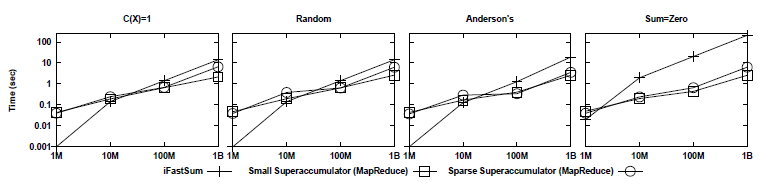
\includegraphics[width=\linewidth]{goodrich_performance}
{\footnotesize \par}
\caption{Total running time obtain by Goodrich and Eldawy \cite{PASFPN} as the input size increases from 1 million to 1 billion numbers}
\end{figure}

\begin{figure}[h]
\centering
\begin{minipage}{0.60\textwidth} % choose width suitably
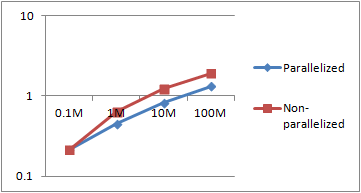
\includegraphics[width=\linewidth]{performance}
{\footnotesize \par}
\end{minipage}
\caption{Performance between 256 threads and 1 thread running on NVidia GTX570 on Windows for N random floating-point numbers}
\end{figure}


In my test I have used an Nvidia GTX 570 processor on a windows machine. The parallized (blue) version of the program used 256 threads while the non-parallelized version used 1 thread per block. As we can see, the parallel version of the algorithm works much better than its sequential counterpart (running 1 thread instead of 256 threads). However, the result is significantly inferior to that obtained by Goodrich and Eldawy This is partly due to the time taken in processing the data into the right format (extracting the mantissa and the exponent). Also the different calculation for the carry bit handling played a role in the result as well.


% ############################################################################
\section{Conclusion} \label{concl}
% ############################################################################

In this project I have implemented a parallelized algorithm for summing large number of floating-point numbers accurately. We have seen that the parallel implementation runs noticeably faster than the non-parallelized implementation of the algorithm. However, because my implementation of $(\alpha, \beta)$ regularization had flaws, I ended up linearly summing the carry bit instead of avoiding it like it was proposed by Goodrich and Eldawy. None-the-less the performance was inferior but comparable to the performance they got in their paper. Since I did not use the exact same machine as they have, it is hard to compare the exact performance difference between my implementations. For further work the $(\alpha, \beta)$ regularization function needs to be fixed for a more accurate performance comparison between the implementations.

% ############################################################################
% Bibliography
% ############################################################################
\bibliographystyle{plain}
\bibliography{my-bibliography}     %loads my-bibliography.bib

% ============================================================================
\end{document}
% ============================================================================
